\chapter{Generator}

There are number solutions that provide formulas in a way of generators or benchmarks:

\begin{itemize}
  \item SMT-LIB \cite{BarFT-RR-17} -- is project aimed at facilitating research and development in \gls{SMT} . One part of their activity is defining syntax for representing formulas in with various theories and hosting considerable benchmark library
  \item SATLIB \cite{Hol00} -- is collection of benchmarks of propositional logic (DIMACS CNF format)
  \item Tough SAT\footnote{\url{https://toughsat.appspot.com/}} -- is a platform that will generate boolean CNF formulas that encode "difficult" problems. Problems are represented in propositional logic (DIMACS CNF format). Although Tough SAT is in fact generator it supports only several predefined problems like Factoring, Subset Sum, Random k-SAT, Cocktail.
% \item PySAT\footnote{\url{https://pysathq.github.io/}} -- is a toolkit, which aims at providing a simple and unified interface to a number of SAT solvers as well as to a variety pseudo-Boolean encodings. Rather than generating benchmarks this tool is useful when there is a need to access several solvers with unified interface.
  \item CNFgen\footnote{\url{https://massimolauria.net/cnfgen/}} -- produces combinatorial benchmarks in DIMACS format. These benchmarks come mostly from research in Proof Complexity (pigeonhole principle, ordering principle, k-clique and more). Many of these formulas encode structured combinatorial problems well known to be challenging for certain SAT solvers.
  \item TSTP (Thousands of Solutions from Theorem Provers) a side project of \gls{TPTP}\cite{Sut17} -- it is a library of problems and solutions encoded in TPTP format
\end{itemize}

Although a lot of ready to use benchmarks can be found, there are not a lot of generators. Tough SAT and CNFgen are generators that generate predefined problem with given size, SMT-LIB, SATLIB, TSTP are mainly repositories of benchmarks, not generators itself. Out of mentioned solutions only SMT-LIB and TSTP support first order logic. None of mentioned solutions can generate first order logic formulas. 

A random first order formula would be useful in this sense, that it would allow creating new datasets with precisely controlled elements. A parameters for such generator shall be described next.

\section{CNF Generator parameters}

User defines generator in 2 steps.

\begin{enumerate}
  \item \textbf{General setting for generated formula}

    In this step user defines set of allowed \gls{FOL} elements:
    \begin{itemize}
      \item set of variable names $\{'v1','v2',\dots\}$
      \item set of functor names $\{'f1','f2',\dots\}$
      \item set of predicate names $\{'p1','p2',\dots\}$
      \item set of allowed functor arities $a_f = \{0, 1, 2,\dots\}$
      \item maximum recursion depth $n$ for functors
      \item set of allowed predicate arities $a_p = \{0, 1, 2,\dots\}$
      \item set of atom allowed connectives, that is no connective or/and any subset of $AllowedConnectives = \{=, !=, \emptyset\}$
      \item set of allowed clause lengths $AllowedClausesLengths = \{1,2,\dots\}$
      \item amount of literals to be negated
    \end{itemize}

  \item \textbf{How many instances of elements are allowed}

    In this step user defines what properties formula should have:
    \begin{itemize}
      \item formula contains from $c_{min}$ to $c_{max}$ clauses
      \item formula contains from $l_{min}$ to $l_{max}$ literals
    \end{itemize}

\end{enumerate}

\section{Intermediate representation}

Abstract syntax tree of \gls{FOL} is implemented in the same way as mathematical definition, see picture \ref{pic:fol_elements_class_diagram}. All classes have base class $FolElement$so that they can be easily identified as element of first order logic and introduce visitor pattern. Visitor pattern is used for exporting formula from intermediate representation to the format of choice (like \gls{TPTP}) as well as counting statistics about generated formula. See for example listing \ref{lis:TPTPExample} - it is convention from TPTP to store some statistics about file at the beginning of file as comment.

Variable and functor are terms, that is why the inherit from term class. Functor is recursive structure it can contain variable or another term, that is why it is connected with aggregation with term class. Predicate can contain only terms, atom can contain term or predicate, literal can contain only one atom but adds sign to it, clause is one or more literal, CNF formula is one or more clause.

\begin{figure}[h]
\begin{centering}
  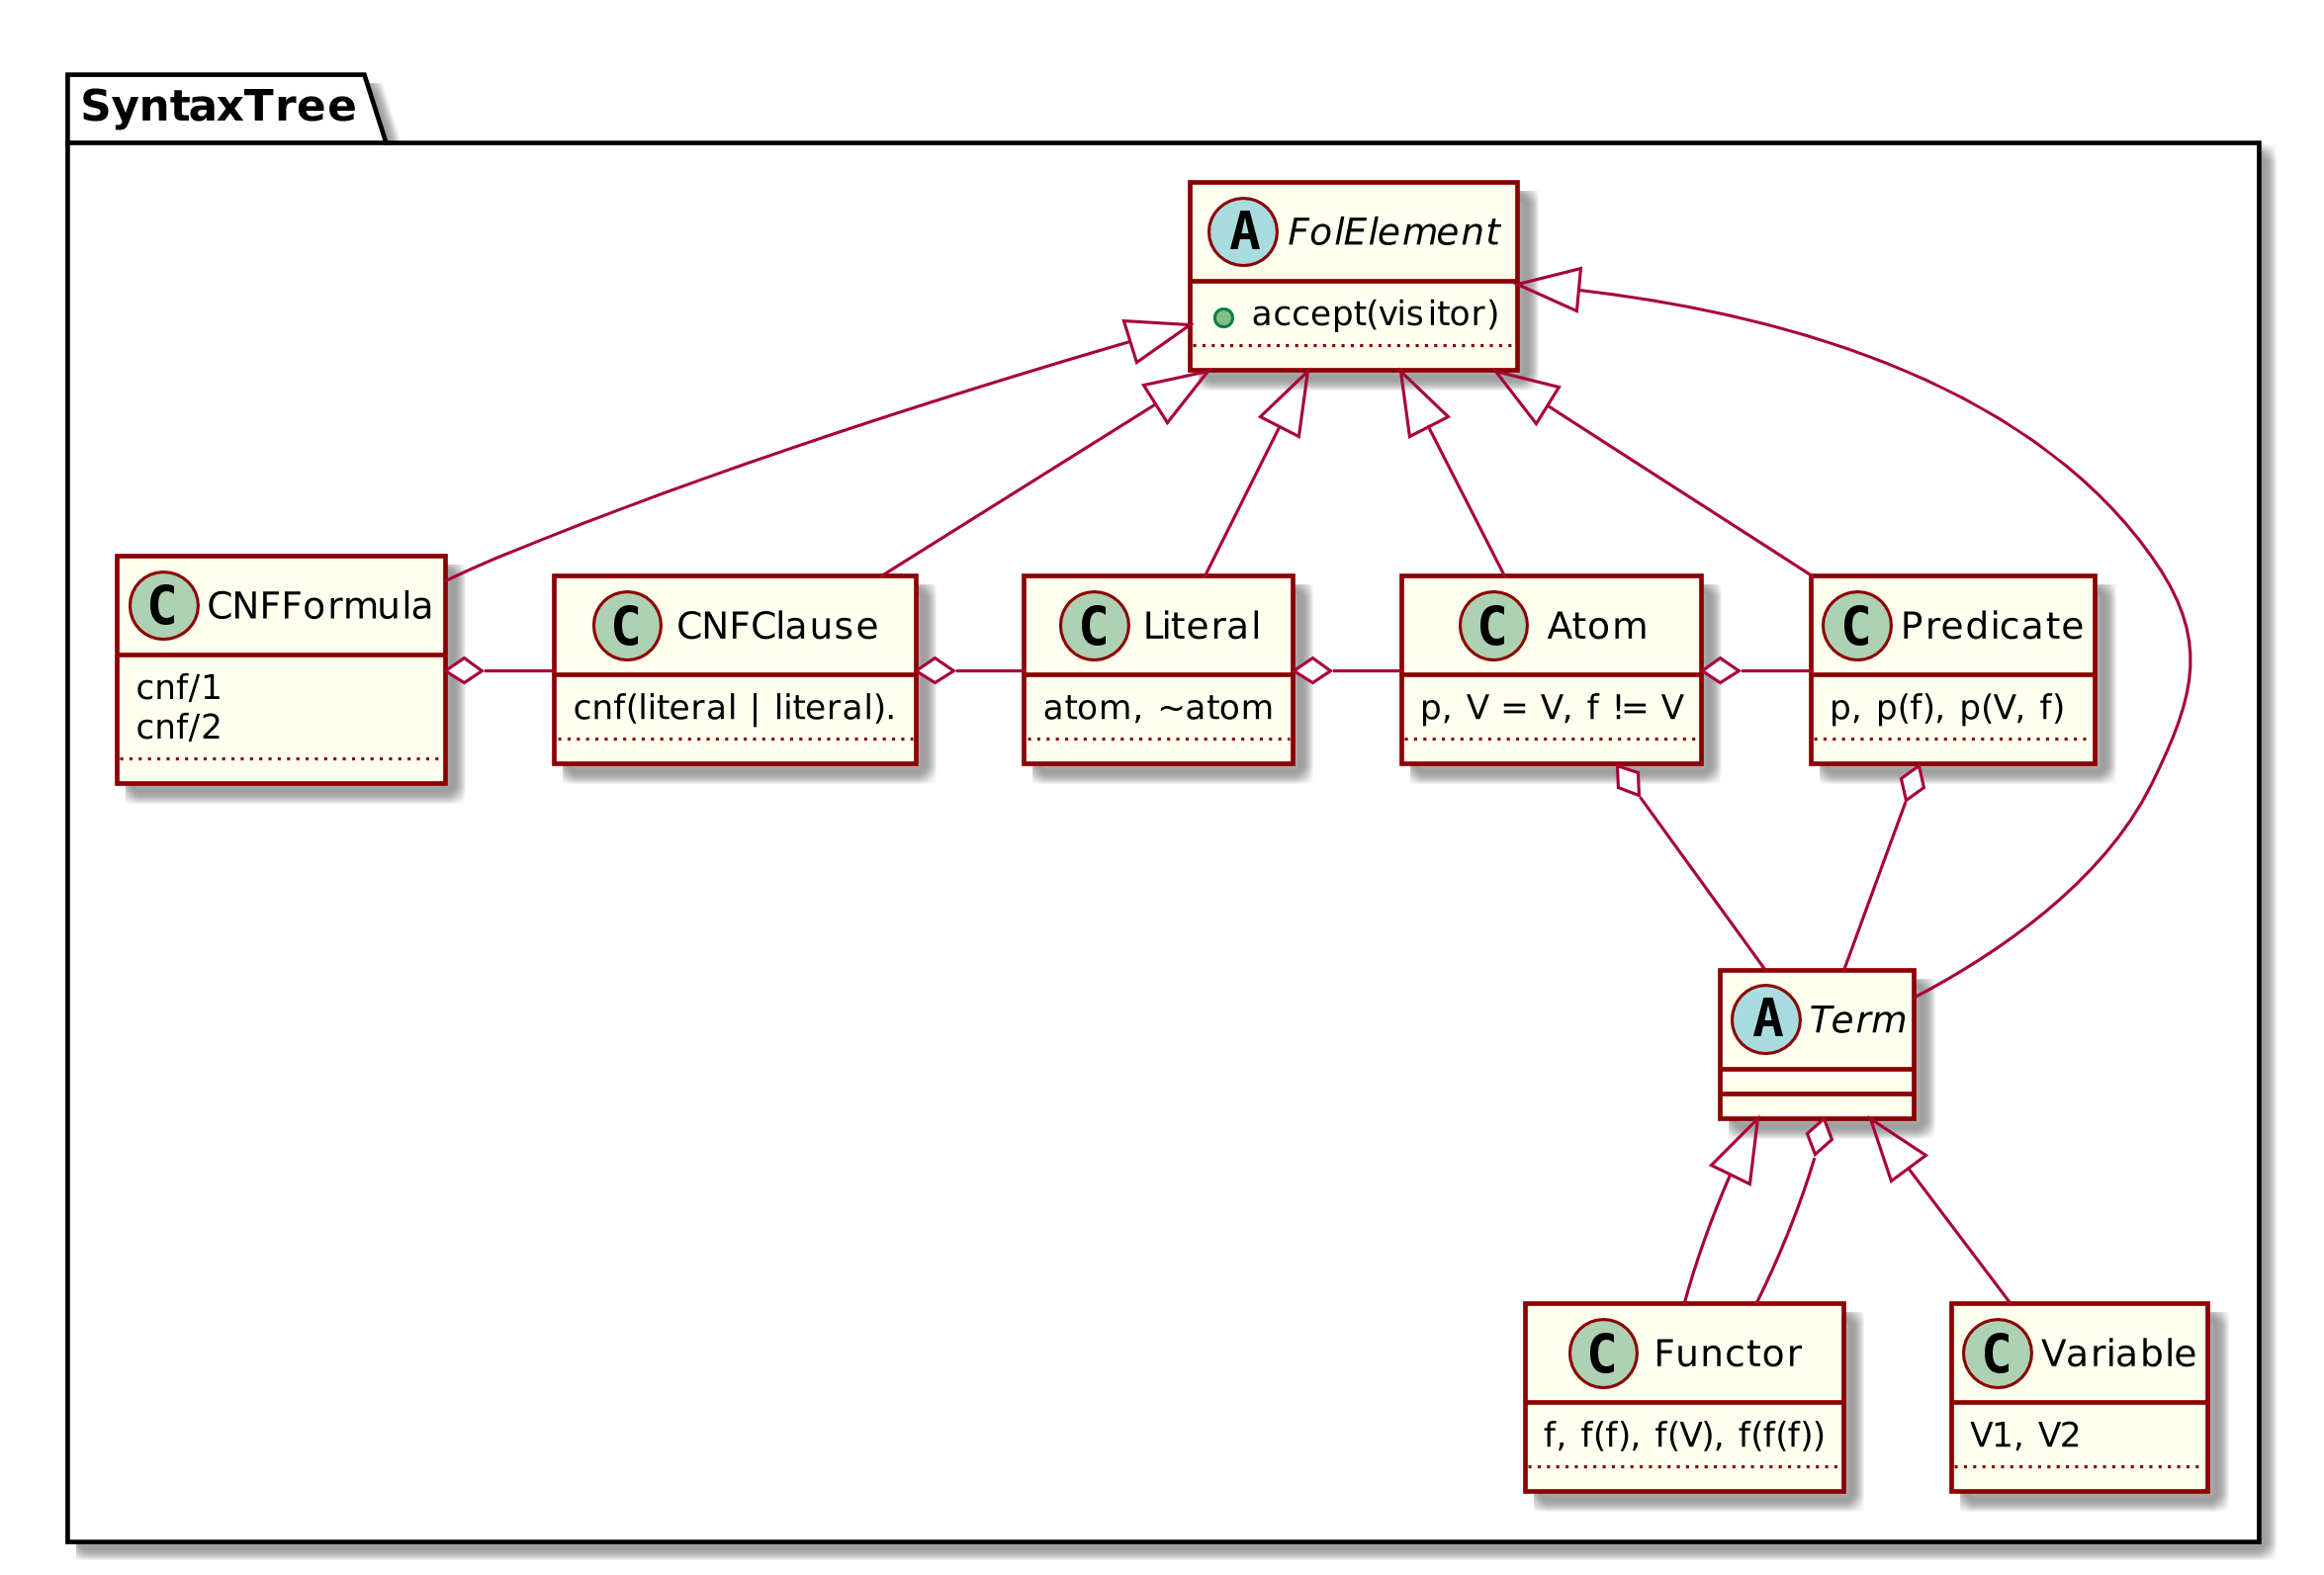
\includegraphics[width=\textwidth]{logic-formula-generator/fol/cnf_fol_elements.png}
  \caption{Class diagram for internal representation of first order logic elements}
  \label{pic:fol_elements_class_diagram}
\end{centering}
\end{figure}
\section{Basic algorithm}

\begin{enumerate}
  \item Resolve user constraints \ref{sec:ResolveUserConstrains}
  \item Generate possible formula based on generators \ref{sec:Generators}
  \item Export formula to file
\end{enumerate}

\section{Resolve user constraints}
\label{sec:ResolveUserConstrains}

User constrains are defined in input parameters as $AllowedClausesLengths$, $NumberOfClauses$, $NumberOfLiterals$. To generate random formula withing these constrains, number of clauses with appropriate clause length must be computed.

CNF formula $F_{cnf}$ consists of unordered clauses $c1, c2, \dots$. 

\begin{align*}
	&F_{cnf}(x) = \{c1, c2, \dots\, cx\} \\
	\text{where }
		&x \text{ -- number of clauses in formula}
\end{align*}

If we group clauses by their length:
\begin{align*}
	&F_{cnf}(x) = \bigcup_{i=1}^c c_i \\
	\text{where }
		&c_i \text{ -- set of clauses with length i} 
\end{align*}

Number of literals in formula can be represented as:
\begin{align*}
	l(x) &= x_1|c_1| + x_2|c_2| + \dots + x_x|c_x| = \sum_{i=1}^{x} x_i |c_i| \\
	x &= x_1 + x_2 + \dots + x_n \\
	c_i &\in AllowedClausesLen: \forall_{i \neq j} c_i \neq c_j  \\
	\text{where }
		&x \text{ -- number of clauses in formula} \\ 
		&l(x) \text{ -- number of literals in formula} \\ 
		&|c_i| \text{ -- number of clauses with length i} 
\end{align*}

So in the end:

\begin{align}
	l(x) &= \sum_{i=1}^{x} x_i |c_i| \\
	x &= \sum_i^x x_i \\
	l_{min} &< l(x) < l_{max} \\
	c_{min} &< x < c_{max} \\
	\text{where } 
		&x \text{ -- number of clauses in formula} \nonumber \\
		&l(x) \text{ -- number of literals in formula} \nonumber  \\
		&|c_i| \text{ -- number of clauses with length i} \nonumber
\end{align}

Solution of above equation are pairs of numbers: clause length and how many clauses with this length should be used in generated clause.

\section{Generators}
\label{sec:Generators}

Generators are implemented as cascade (picture \ref{pic:fol_signature_generator_class_diagram}), that is formula generator provides formulas, but requires clause generator, clause generator provides clauses, but requires literal generator and so on.

\begin{figure}[h]
\begin{centering}
  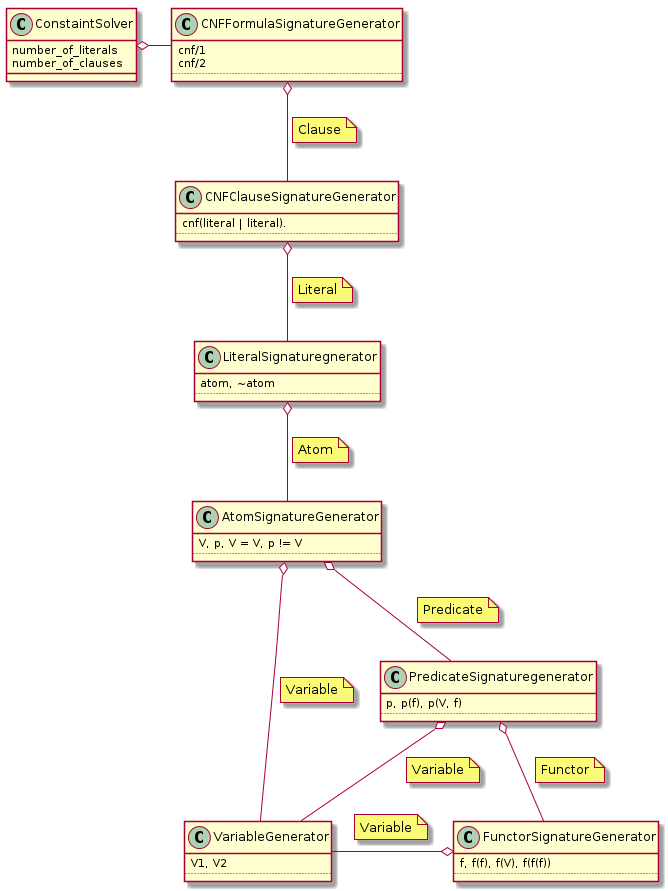
\includegraphics[width=0.7\textwidth]{logic-formula-generator/fol/cnf_signature_generators.png}
  \caption{Class diagram of generators in CNF formula generator}
  \label{pic:fol_signature_generator_class_diagram}
\end{centering}
\end{figure}

Manual creation of generators is required only in advanced case. To automate this process $CNFFormulaGnerator$ (picture \ref{pic:cnf_generator_class_diagram}) has been created. This is interface for user to create random CNF formulas that will automatically resolve user constraints and yield random formula. After creating formula from signature generators formula will be post processed - given random names and optionally negation sign. Generated formula can be then exported to file along with statistics about formula.

\begin{figure}[h]
\begin{centering}
  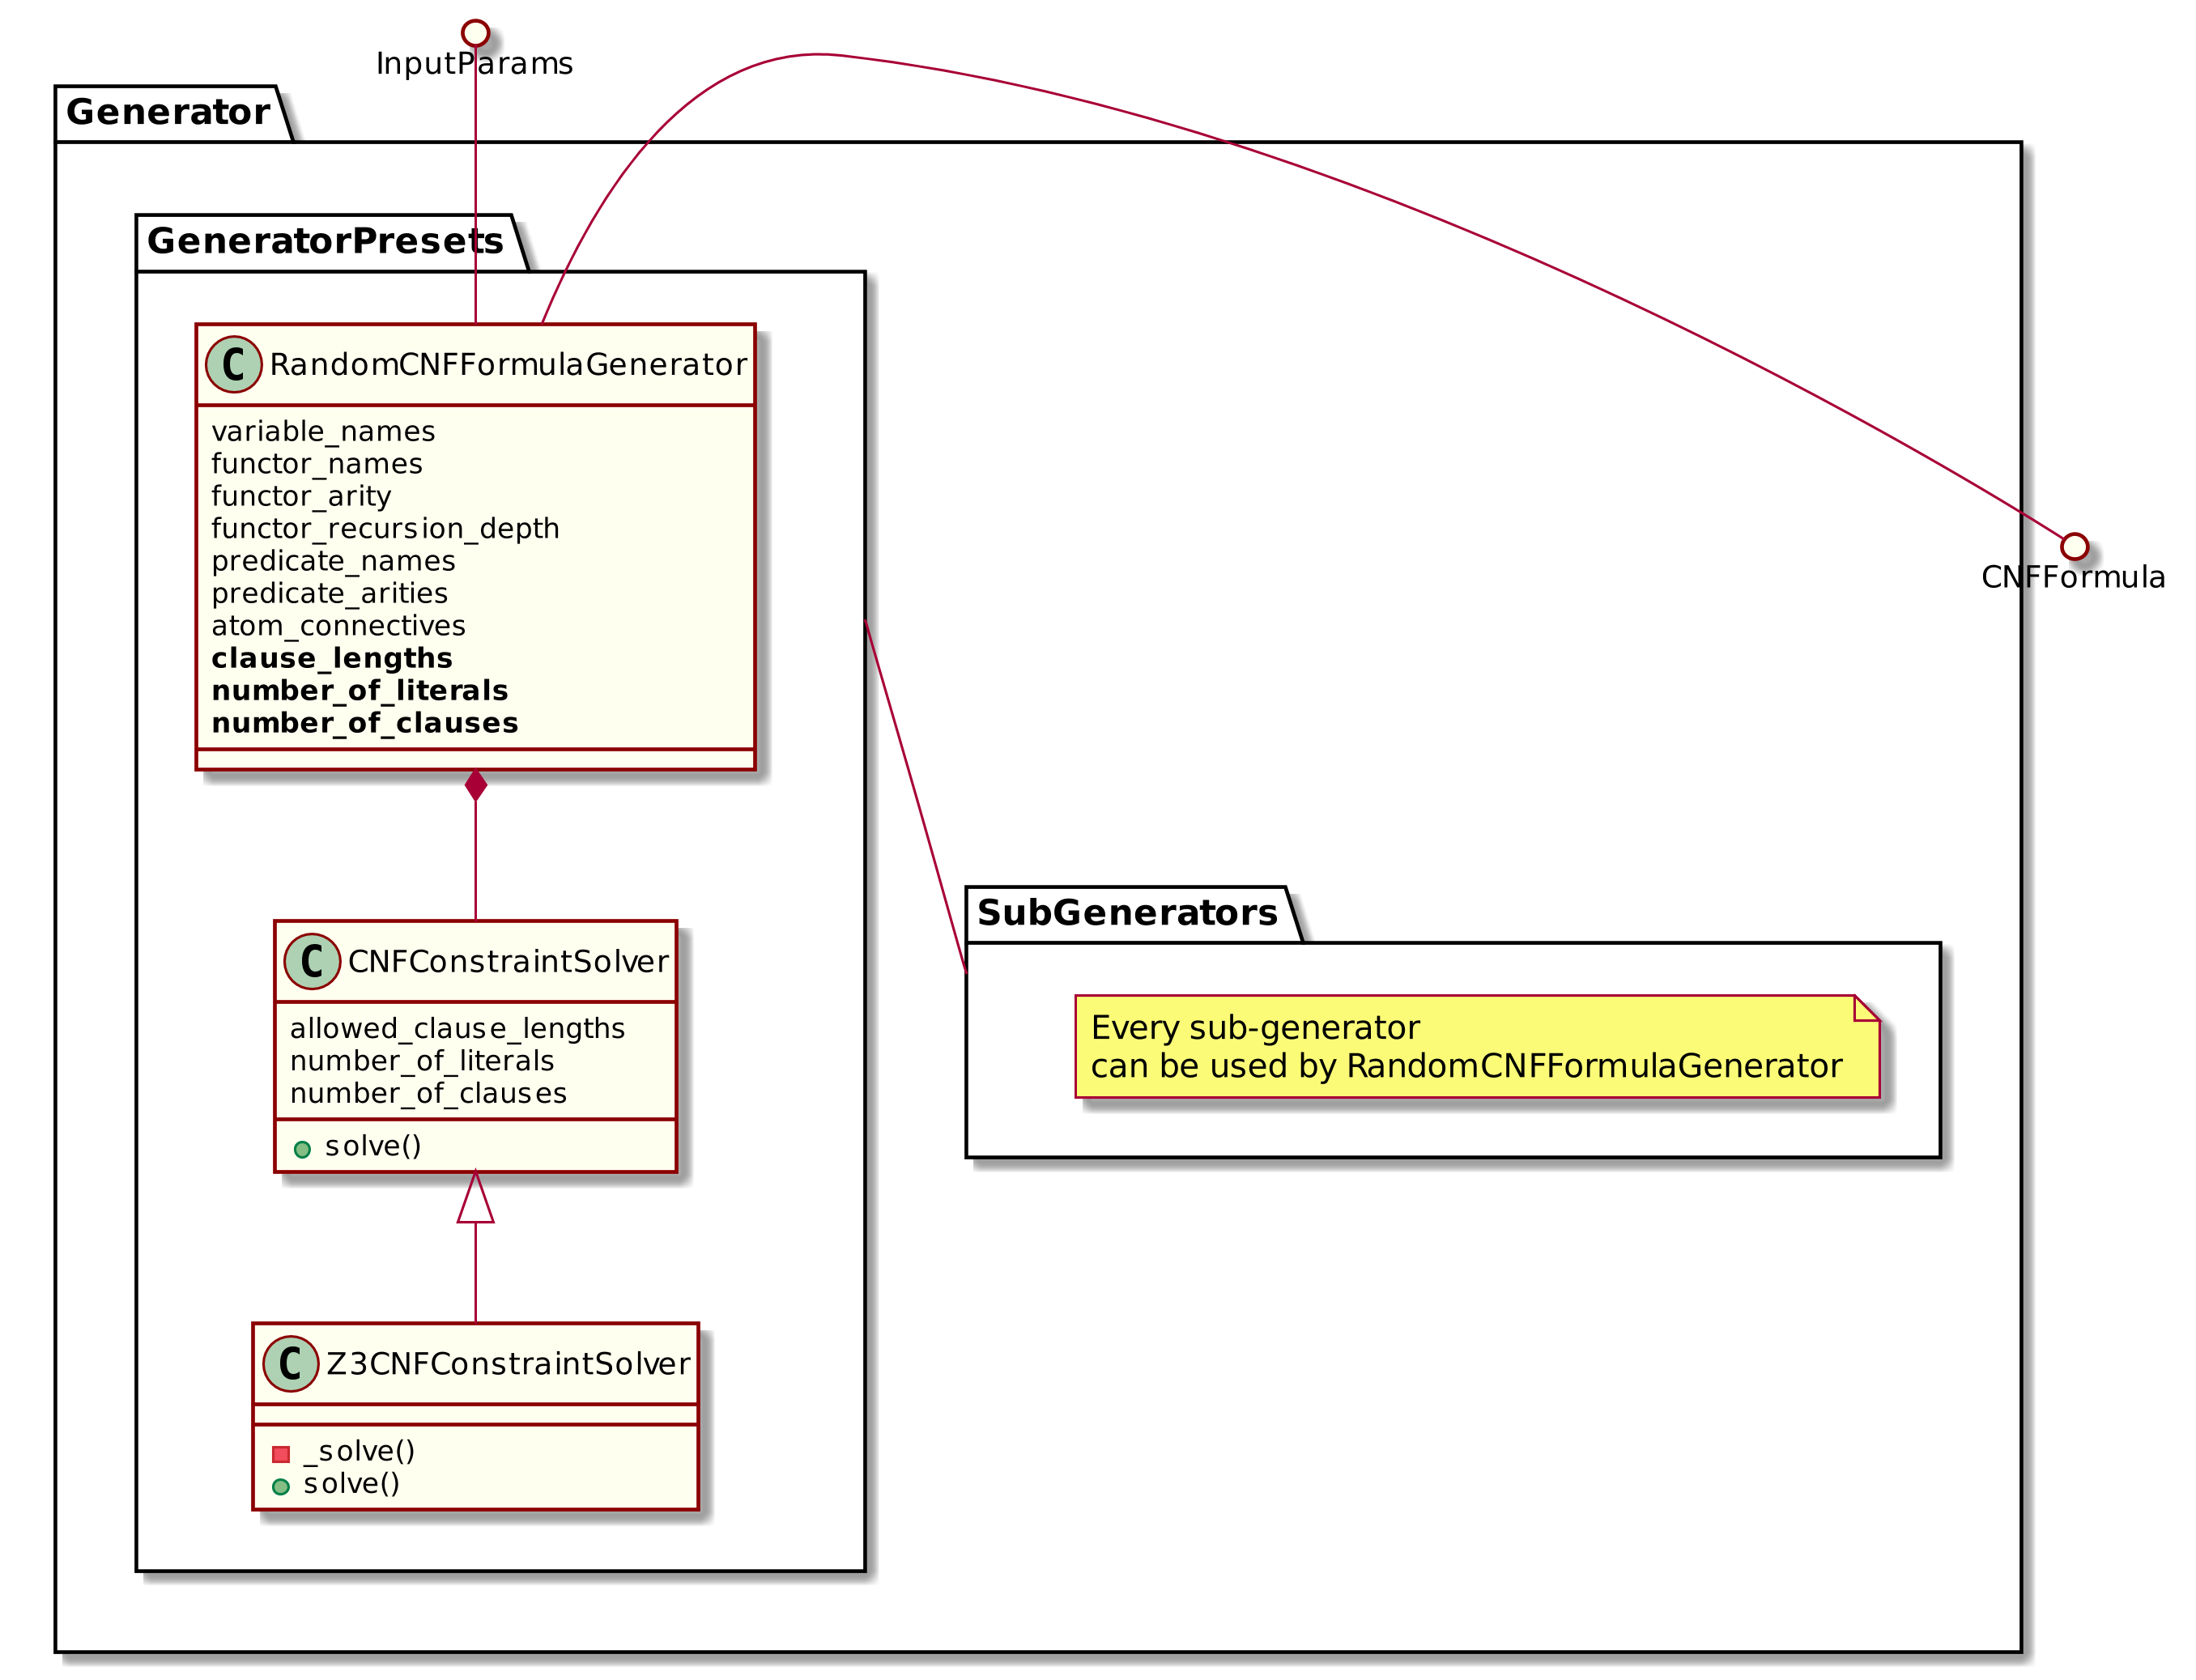
\includegraphics[width=\textwidth]{logic-formula-generator/cnf_formula_generator.png}
  \caption{Class diagram of CNF formula generator}
  \label{pic:cnf_generator_class_diagram}
\end{centering}
\end{figure}

